\documentclass[citeauthoryear]{llncs}
\usepackage{url}
\usepackage{cite}
\usepackage{listings}
\usepackage[utf8]{inputenc}
\usepackage{graphicx}
\usepackage{float}
\usepackage{verbatim}
\usepackage{eurosym}


%\title{Assessing Modeling Languages, metrics and tools}
\title{Modeling Languages: metrics and assessing tools}

%Exemplo para adição dos autores
\author{Daniela Fonte \and Ismael Vilas Boas \and José Azevedo \and José João Peixoto \and Pedro Faria \and Pedro Silva \and Tiago Sá \and  Ulisses Costa \and Daniela da Cruz \and Pedro Rangel Henriques}

\institute{Department of Informatics, University of Minho\\ Campus de Gualtar, 4710-057 Braga, Portugal\\
\email{\{danielamoraisfonte, ismael.vb, jazevedo, jj.peixotopereira, pedro.faria.80, zepedro.cs, ulissesmonhecosta, danieladacruz, pedrorangelhenriques\}@gmail.com, tiago@esterisco.com}
}

\newcommand{\uml}{\textsf{UML}}
\newcommand{\xmi}{\textsf{XMI}}
\newcommand{\xml}{\textsf{XML}}
\newcommand{\entArch }{\textsf{Enterprise Architect}}
\newcommand{\sdmetrics}{\textsf{SDMetrics}}

\begin{document}
\maketitle

%%Abstract
\begin{abstract}
Any traditional engineering field has metrics to rigorously assess the quality of their products.
From a long time ago, engineers know that the production process is not all; the output must comply with 
the rules and good-practices, must satisfy the requirements and must be competitive.\\
Professionals in the new field of software engineering started a few years ago  to define metrics to appraise 
their product: individual programs and software systems.\\
This concern motivates the need to assess not only the outcome but also the process and tools employed in its development.
In this context, assessing the quality of programming languages is a legitimate objective;
in a similar way, it makes sense to be concerned will models and modeling approaches, as more and more
people starts the software development process by a modeling phase.\\
In the paper we discuss the quality of modeling languages, introducing and motivating the topic,
presenting metrics, and comparing tools.
\end{abstract}

\keywords Modeling Languages, Software/Language Quality, Software/Language Metrics, UML

%%Introdução
\section{Introduction}

\indent
\par A model is a representation of reality aiming at the simplification of some complex object.

\par Models are built so that we can better understand the system being developed.
They help us to visualize a system as it is or as we need it to be. Models allow us to specify the structure and behavior of a system, they provide the guidance lines/blueprints in constructing a system, and finally, models document the decision taken for a given system;


\par Some models are best described textually, other graphically. All interesting systems exhibit structures that transcend what can be represented in a programming language.


\par A modeling language is a language whose vocabulary and rules focus on the conceptual and physical representation of a system.%%todo

\par Specifying means building models that are precise, unambiguous and complete. 

The \umlS~addresses the specification of all the important analysis, design and implementation decision. %todo

%% prh idea
\par One the one hand, one can produce a strict formal specification of the system, which allows us to reason over the system proprieties, without running the system.
On the other hand, one can follow a pragmatic aproach, using a diagramatic specification of the system, not allowing us to reason over programs,
but deriving programs from the model specification. That aside, when assessing a modeling language we might infer on its quality.
\begin{quotation}
Effective management of any process requires quantification, measurement, and modeling.
Software metrics provide a quantitative basis for the development and validation of models of the software development process.
Metrics can be used to improve software productivity and quality\cite{g1:Millis:1998}.
\end{quotation}

The main goal to use model/software metrics is to be able to generate quantifiable measurements from the specifications/software. The use of model metrics is even more
important to numerous valuable applications in earlier stages of the development process: in scheduling, cost estimation, quality assurance, and personnel task assignments.

\begin{quotation}
Effective management of any process requires quantification, measurement, and modeling.
Software metrics provide a quantitative basis for the development and validation of models of the software development process.
Metrics can be used to improve software productivity and quality\cite{g1:Millis:1998}.
\end{quotation}
    
Nowadays, metrics become increasingly essential for Software Engineering: they are crucial for quality assessment and reengineering processes.
In \emph{Forward Engineering} they are used to measure the software quality and estimate cost and effort of software projects\cite{Fenton}.
In the field of \emph{Software Evolution}, they can be both used to identify stable or unstable parts of a system as to determine where refactoring can be or have been applied\cite{Serge}.
They even can be used for assessing the quality and complexity of software systems in \emph{Software Reengineering} or \emph{Reverse Engineering}\cite{43044}.

When focusing on the field of Object-Oriented (OO) systems, many metrics have been proposed for assessing the design of a software system.
However, most of the existing approaches involve the analysis of the source code and cannot be applied in earlier stages of the development process.
In fact, it is not always simple to apply the existing metrics in this earlier stages. 
As the \textsf{Unified Modeling Language}, proposed by Booch, Jacobson and Rumbaugh\cite{USDPuml} has became a standard for expressing OO systems, apply metrics to these models enables an early estimate of development efforts, implementation time, complexity and cost of the system under development. \\

In this paper, we will introduce and discuss the major existing metrics for \umlS~models, and focus on present a set of tools designed for measure \umlS~projects.
In what follows, Section~\ref{metrics} we describe the principal measurements applicable to the most popular \umlS~diagrams.
In Section~\ref{tools} we present two of the best tools designed to extract metrics from \umlS~models and the results of applying them a real case-study.
Then, Section~\ref{assess} is devoted to the metrics assessment process.
We conclude in Section~\ref{conc} with a comparsion between the presented tools.


%%Metrics intro
\section{Applying Metrics To \uml\ Models}\label{metrics}

An \uml\ model can be made from different diagrams, each one with a distinct view of the system.
We have, in one hand, Use Cases diagrams which expose the system functional requirements and how each user interacts with them. They are a good overview of what features the system offers to the end user.
In the other hand, we use Class Diagrams for represent the blueprint of the application under the developer perspective: they illustrate which programming components a system has and how they related to each other.
Package Diagrams describe how to group the classes and how these groups relate to each other (\textit{package import}, \textit{package merge}).
%We believe that an \uml\ diagram need to have at least these three diagrams implemented, because they give to both the costumer and the developer the full knowledge of the system.
Here we present some metrics related to this three fundamental diagrams and conclude the section by introducing some metrics for other not less important \uml\ diagrams.


%%ck metrics
\subsection{Object-Oriented Software: \textrm{CK} Metrics}
One of the most popular suites of OO metrics was proposed by Chidamber and Kemerer \cite{Chidamber:1994:MSO:630808.631131}.
They were proposed to capture different aspects of object-oriented designs, including complexity, coupling and cohesion,
and were posteriorly adapted for modeling languages as we can see in~\cite{Power2}.

This suite is composed by six metrics: Weighted Methods Per Class (WMC), Depth of Inheritance Tree (DIT), Number of Children (NOC), Coupling between Object Classes (CBO), Response For a Class (RFC), e Lack of Cohesion in Methods (LCOM).
We detail bellow each metric and its features.\\

\paragraph{Weighted methods per class} (WMC): This metric regards to the complexity of a class's methods, being equal to the sum of the complexities of those methods defined. There two kinds of WMC metrics:
\begin{itemize}
\item \textbf{$WMC1_{1}$} can be obtained from a class diagram of a \umlS model. It is computed by identifying the class and counting the number of methods in that class, which means that, in this case, the WMC metric considers a method as a unity.
\item \textbf{$WMC_{cc}$} is also computed by identifying the class and counting the number of methods, but each method is not a unity, is the result of a McCabe Cyclomatic Complexity of it. Another difference is that this kind of WMC cannot be computed only with information of diagrams class, needing information of other kinds of diagrams, like sequence or activity.
\end{itemize}

\paragraph{Depth of inheritance tree} (DIT): This metric is equal to the maximum length from the class to the root of the inheritance, which could be defined as the depth of the class. It is computed by taking the union of all the class diagrams in a \umlS model and traversing the inheritance hierarchy of the class.

\paragraph{Number of children} (NOC): This metric represents the number of childs and descendants of a certain class. Can be obtained gathering all diagrams class, in a \umlS modulation, and checking all the inheritance relations of the class.

\paragraph{Coupling between object classes}: Two classes are related if the method of a class uses a instance variable or method of another class. Counting the number of classes to which the class are related and counting all kind of references of the attributes and parameters of the methods of the class, an estimate of this metric's value can be obtained from the class diagrams. Though, it is possible to calcute a more precise value if the behavioural diagrams are taken into account, since the usage of instance variable and invocation methods are additional information.

\paragraph{Response for a class} (RFC) - This metric is the number of methods that can be invoked by an object of a given class. It can be obtained from a class diagram and, also, by behaviour diagrams (e.g. sequece diagrams), which can inform of several methods of other classes that are invoked by each of the class's methods.

\paragraph{Lack of cohesion in methods} (LCOM)- Is the metric that measure the number of sets of instance variables accessed by every pair of methods, of a given class, that has a non-empty intersection. With the intention of computing a value for this metric, it is essential the information of the usage instance variables by the methods of a class, i.e., it is needed a sequence diagram (a class diagram does not have information about the usage).

The set of metrics that were here defined can be found and cited in several papers (probably the most famous~\cite{Power2}). They are currently the most studied and used to evaluate \uml models.\\


%%Diagram class metrics
\subsection{Class Diagram and Package Metrics}

These diagrams are used to describe the types of objects in a system and the relationships among them.
They describe the structure of a system by showing the system classes, their attributes and methods or operations.
Their quality have a huge impact on the final quality of the software under development, as they describe the general model of the system information.

\begin{table}
\begin{minipage}[b]{0.5\linewidth}\centering
\begin{tabular}{ p{1,5cm} | p{4cm}}
\multicolumn{2}{l}{\textbf{Marchesi Metrics}} \\ \hline
\textbf{Metric} & \textbf{Description} \\ \hline
NC & Number of Classes \\ \hline
CL1 & Weighted Number of Class responsibilities   \\ \hline 
CL2 & Weighted Number of Class Dependencies \\ \hline 
CL3 & Depth of inheritance tree \\ \hline 
CL4 & Number of immediate subclasses of a given class \\ \hline 
CL5 & Number of distinct class \\ \hline 
\end{tabular}
\caption{\small{Marchesi Class Diagram Metrics}}
\label{t:dcm}
%\end{table}
%\end{center}
\end{minipage}
\hspace{0.3cm}
\begin{minipage}[b]{0.5\linewidth}
\centering
%\begin{center}
%\begin{table}[h]
\begin{tabular}{ p{1,5cm} | p{4cm}}
\multicolumn{2}{l}{\textbf{Marchesi Metrics}} \\ \hline
\textbf{Metric} & \textbf{Description} \\ \hline
NP & Number of Packages. \\ \hline 
PK1 & Number of Classes \\ \hline
PK2 & Weighted Number of responsibilities of a Class   \\ \hline 
PK3 & Overall Coupling among Packages \\ \hline 
\end{tabular}
\caption{\small{Marchesi Package Metrics}}
\label{t:pcm}
%\end{table}
%\end{center}
\vspace{0.78cm}
\end{minipage}
\end{table}

Measures like the \emph{Number of Attributes in the Class}, the \emph{Number of Operations in the Class}, \emph{Number of Inherited Attributes}, \emph{Number of descents/ancestors of a Class}, or even the \emph{Number of Interfaces Implemented} are used both for indicate the system complexity and as an index of quality.
Many works present several metrics for this diagrams~\cite{DBLP:journals/Lobjet/GeneroPC00},~\cite{Eichelberger_onclass},~\cite{Yi04acomparison}.
The OOA metrics defined by Marchesi~\cite{Marchesi:1998:OMU:522081.795010} also contemplate Class Diagrams, as we can see in Table~\ref{t:dcm}.


In UML, classes can be grouped into Packages to define subsystems or even for implementation purposes.
The measurement of a package complexity is useful to forecast the development efforts of it.
For that, we can measure properties like the \emph{Number of Classes of a Package}, the \emph{Total Number of Packages in the system}, or the \emph{Number of Interfaces in the Package}.
Marchesi~\cite{Marchesi:1998:OMU:522081.795010} suggests several Package Metrics as we can see in Table~\ref{t:pcm} that allow to estimate this complexity.


%%Use Case metrics
\subsection{Use Case Metrics}

The Use Cases Diagrams are graphical representations of entities which interact with the system - the \emph{actors}, and operations that the system must perform for them.
They define a sequence of actions which illustrate a specific way of using the system.

These diagrams are functional specifications, collected at the beginning of a system development process.
They are crucial to an early estimate of the system complexity and its development efforts, as we can see by the UC metrics defined in several works like~\cite{Kim02developingsoftware},\cite{Mohagheghi05effortestimation}, \cite{Ribu01estimatingobject-oriented}.

In fact, measuring the number of Use Cases, actors and communications among them is a good indicator of the system complexity, as well as to quantify the relationship between diagrams (i.e. estimates the number of UC that extend or include others).

One remarkable work on this area was performed by Michele Marchesi~\cite{Marchesi:1998:OMU:522081.795010}.
Table~\ref{t:ucm} illustrates the Use Case metrics defined on this work. 
 
\begin{table}[h]\centering
\begin{tabular}{ p{1,5cm} | p{10.5cm}}
\multicolumn{2}{l}{\textbf{Marchesi Metrics}} \\ \hline
\textbf{Metric} & \textbf{Description} \\ \hline
NA & Number of actors of the system. \\ \hline
UC1 & Number of Use Cases in the system. \\ \hline 
UC2 & Number of communications among UC and Actors  \\ \hline 
UC3 & Number of communications among UC and Actores without redundancies \\ \hline 
UC4 & Global complexity of the system \\ \hline 
\end{tabular}
\caption{\small{Marchesi Use Case Metrics}}
\label{t:ucm}
\end{table}

The \textbf{UC4} metric represents a balance of the global complexity of the system, and its value is obtained through the values of \textbf{UC1}, \textbf{UC2} and \textbf{UC3} metrics.

%%Other
\subsection{Other Metrics}

Statechart diagrams illustrate the behavior of an object.
They define different states of an object during its lifetime, which are changed by events.
A \emph{state} expresses an action of an object during a certain time, when it don't receive external stimulus nor is there any change in its attributes. 

\begin{table}[h]\centering
\begin{tabular}{ p{2cm} | p{10,5 cm}}
\multicolumn{2}{l}{\textbf{Métricas de Estados}} \\ \hline
\textbf{Métrica}  & \textbf{Descrição} \\ \hline
TEffects  & The number of transitions with an effect in the state machine. \\ \hline 
TGuard & The number of transitions with a guard in the state machine. \\ \hline 
TTrigger & The number of triggers of the transitions of the state machine. \\ \hline 
States & The number of states in the state machine. \\ \hline 
\end{tabular}
\caption{\small{Exemplos de Métricas sobre Diagramas de Estados}}
\label{t:estado}
\end{table}

Measures like the \emph{Number of Entry Actions}, \emph{Number of Exit Actions}, \emph{Number of Transitions}, or even the \emph{Number of Activities} are associated to the complexity and dimension of the problem~\cite{EVMmdm}.
In Table~\ref{t:estado} we can notice some examples from measurable attributes for this type of diagram.

Activity diagrams describe work flows and are very useful for detail operations of a class (including behaviors expressed by parallel processing).
As we can see in Table~ref{t:act} several metrics for this diagrams are available.

\begin{table}[h]\centering
\begin{tabular}{ p{2cm}|   p{10,5 cm}}
\multicolumn{2}{l}{\textbf{Métricas de Actividade}} \\ \hline
\textbf{Métrica} & \textbf{Descrição} \\ \hline
Actions  & The number of actions of the activity. \\ \hline 
ObjectNodes & The number of object nodes of the activity. \\ \hline 
Pins  & The number of pins on nodes of the activity. \\ \hline 
Guards  & The number of guards defined on object and control flows of the activity. \\ \hline 
\end{tabular}
\caption{\small{Exemplos de Métricas sobre Diagramas de Actividade}}
\label{t:act}
\end{table}

Besides these metrics, it is possible to measure attributes like the \emph{Number of Activity Groups/Zones}, the \emph{Number of object flows} or even the \emph{Number of Exceptions} of each diagram. 
%%Tools
\section{Tools for UML Metrics Calculation} \label{tools}

Nowadays, the most popular UML tools for software application development are \textsf{Visual Paradigm for UML\footnote{Available at \url{http://www.visual-paradigm.com/product/vpuml/}}} and \textsf{Poseidon for UML}\footnote{Available at \url{http://www.gentleware.com/products.html}}.
They enable a visual environment to model software, which reduces the complexity of software design.
However, they not support metrics specification - it is required to use other tools, designed for this task.
In the next subsections, we will introduce the leading systems on the quantitative analysis of UML models structural properties, and put them to test for explore their features with a real case-study.

One of the tools that we are going to address is SDMetrics\footnote{SDMetrics can be found at \url{http://www.sdmetrics.com/}}, a design measurement tool for UML models.
%SDMetrics is not free so we required an academic license from the staff, which was quickly provided. 
%Its core is open source and is available under the GNU Affero General Public License.
Although its core is open source and available under the GNU Affero General Public License, SDMetrics GUI it is not freely distributed. 
In order to explore all the system features, SDMetrics staff gently provided us an Academic License which we sincerely would like to thank.

The core functionalities of SDMetrics include:
\begin{itemize}
\item the configurable XMI parser for XMI1.0/1.1/1.2/2.0/2.1 input files;
\item the metrics engine to calculate the user-defined design metrics;
\item the rule engine to check the user-defined design rules.
\end{itemize}


The other tool we put to test is the \textsf{Sparx System Enterprise Architect}{\footnote{\url{http://www.sparxsystems.com.au}}}, a team-based modeling environment. 
It embraces the full product development lifecycle, supporting both software design, requirements management, and metrics calculation for Use Case Diagrams.
Thus, it allow to estimate the complexity of the project in a earlier stage, as well as the complexity associated with each actor of the system.

%%Case Study
\subsection*{Case Study}

The case-study used to explore this tools is the modelation made for a project of a subject during our graduation. The subject name was Software Systems Development and it's project was \textit{MWK (Manages With Knowledge)}.\\
In the project, MWK is a company which doesn't provide services, but on the other hand, to meet it's clients needs, it has a wide range of suppliers, that MWK subcontracts, who are responsible for the service execution. Multiple suppliers can supply the same service and each  service can be delivered in different ways. Each service can then be composed of multiple activities. As an example, there could be a service called \textit{Shirts til 10Kg} and inside this service there could be activities such as \textit{wash, iron, sewing buttons, etc}.\\
Each activitie of a given service as a stipulated price, and can be hired by a client.\\
The goal of the project was to model and implement a management software, with the same name as the company, that would help the completion of all the tasks inherent to the company.\\

As an example of the UML diagrams used on the test, we will display one image of the general Usecase diagram and an excerpt of the class diagram.

\begin{figure}[H]
\begin{center}
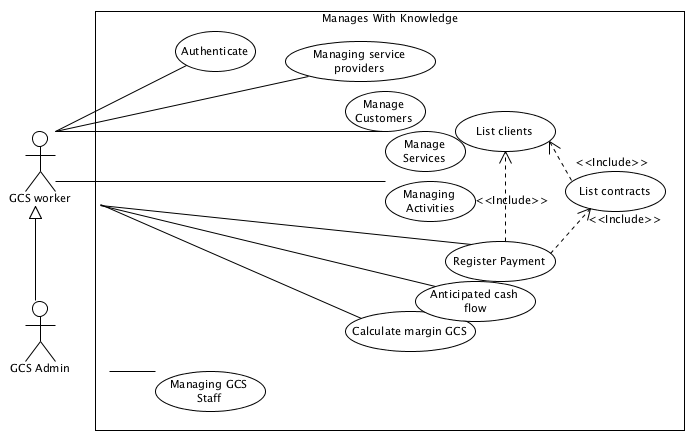
\includegraphics[width=0.9\textwidth]{images/usecase.png}
\caption{The general Usecase of the modelation}\label{img:usecase}
\end{center}
\end{figure} 

\begin{figure}[H]
\begin{center}
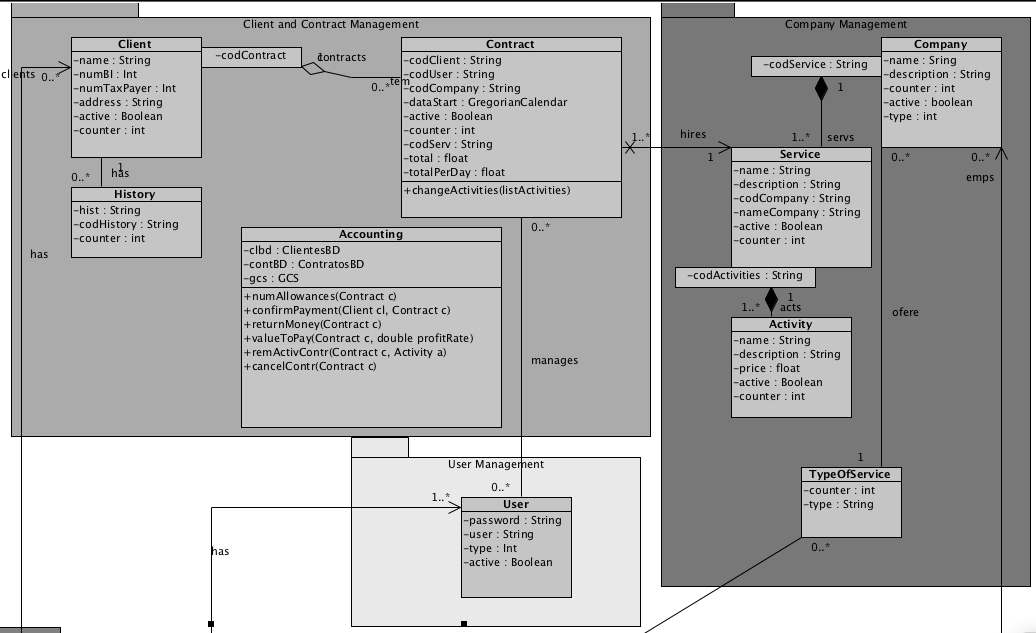
\includegraphics[scale=0.35]{images/classbw.png}
\caption{Excerpt of the Class diagram}\label{img:class}
\end{center}
\end{figure} 

%SDMetrics
\subsection{SDMetrics}
SDMetrics is a very complete design measurement tool, analysing a wide range of UML diagrams, including Class, Usecase, Activity and Statemachine diagrams.
For each type of diagram, this tool generates several metrics.\\
For example, \textbf{NumAttr} metric, one of the metrics that has already been adressed in this paper, is calculated from Class diagrams.
Other one is \textbf{ExtPts}, wich is calculated from Usecase diagrams, and gives us the number of extension points of a given use case.\\

SDMetrics is written in java, and provides us a graphical user interface. The type of source files it receives to analyse are \textit{XMI}\footnote{
\textit{XMI} (\textbf{X}ML \textbf{M}etadata \textbf{I}nterchange)  is an \textit{OMG} (Object Management Group) standard to generate
XML-based representations of UML and other OO data models.} files, most modeling tools support project exportation in XMI.\\
This tool allows us to access the results from different views. We will approach the ones that seem the most important:
\begin{itemize}
\item \textbf{Metric Data Tables} provides a table that matches each UML model element analysed (table line) to it's value for each metric (table column);
\item \textbf{Histograms} provides a graphical distribution  for each design metric;
\item \textbf{Design Comparison} provides us a mean to compare the structural properties of two \textit{UML} designs. It is very useful to compare the same design in different iterations of the development, or to compare an alternative design to the current one.
\item \textbf{Rule Checker} design rules and heuristics detect potencial problems in the UML design such as: 
	\begin{itemize}
	\item incomplete design such as unnamed classes, states without transitions;
	\item violation of naming conventions for classes, attributes, operations, packages;
	\item etc.
	\end{itemize}
\item \textbf{Catalog} this view provides us with the definitions of the metrics, design rules, and relation matrices for the current data set, and provides literature references and a glossary for them.
\end{itemize}
Not a view, but one of the most advanced features in this software is the possibility of defining Custom Design Metrics and Rules. The new metrics are defined in a XML file, with a very particular format, the \textit{SDMetricsML} (SDMetrics Markup Language). \\
The SDMetrics tool doesn't provide a direct notion of good/bad quality of the design model. Despite that, on the SDMetrics website we can find several indications of how to interpret each kind of metrics. 
 
\subsubsection{Results}

Next we will show some printscreen's taken from SDMetrics, which will illustrate some of the outputs of this software, for our case-study.\\

\textbf{Metrics Table}
\begin{figure}[H]
\begin{center}
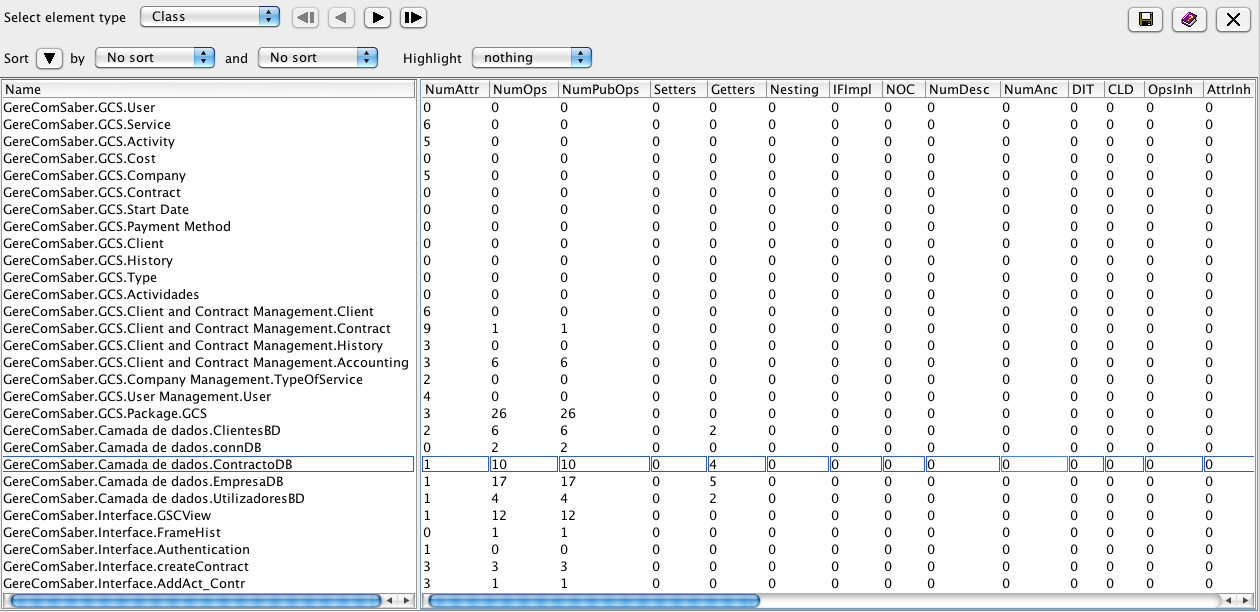
\includegraphics[width=1\textwidth]{images/table.png}
\caption{Metrics Table for class diagrams}\label{img:table}
\end{center}
\end{figure} 

\textbf{Histogram}
\begin{figure}[H]
\begin{center}
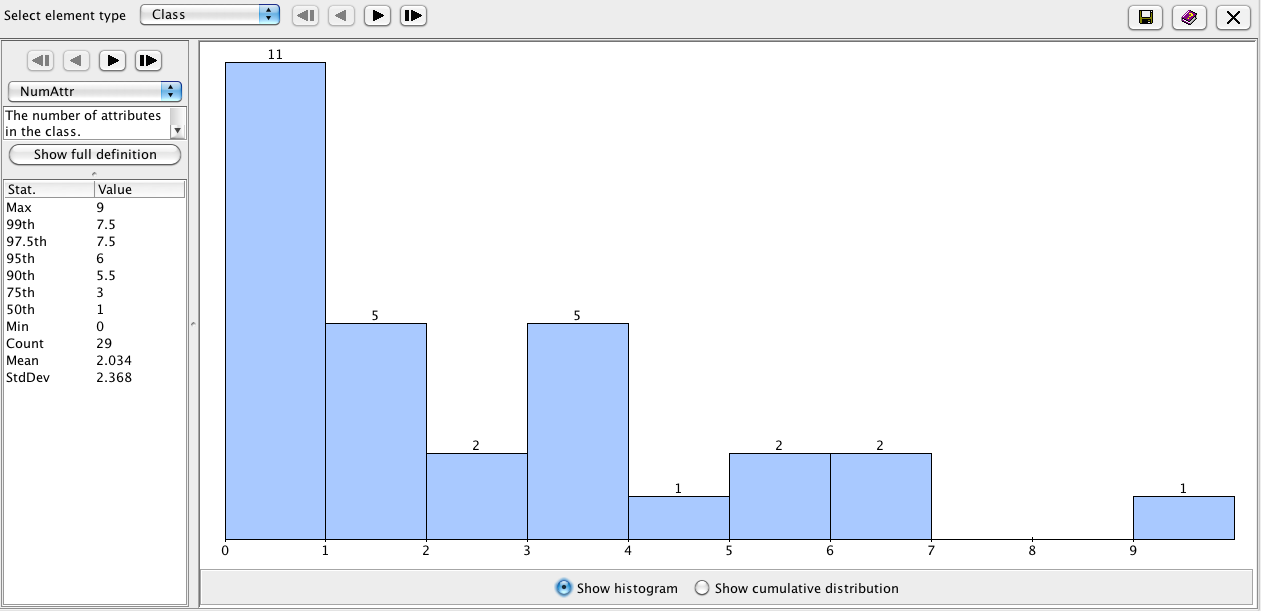
\includegraphics[width=1\textwidth]{images/histogram.png}
\caption{Histogram for class diagrams evaluating the metric NumAttr}\label{img:histogram}
\end{center}
\end{figure} 

\textbf{Rule Checker}
\begin{figure}[H]
\begin{center}
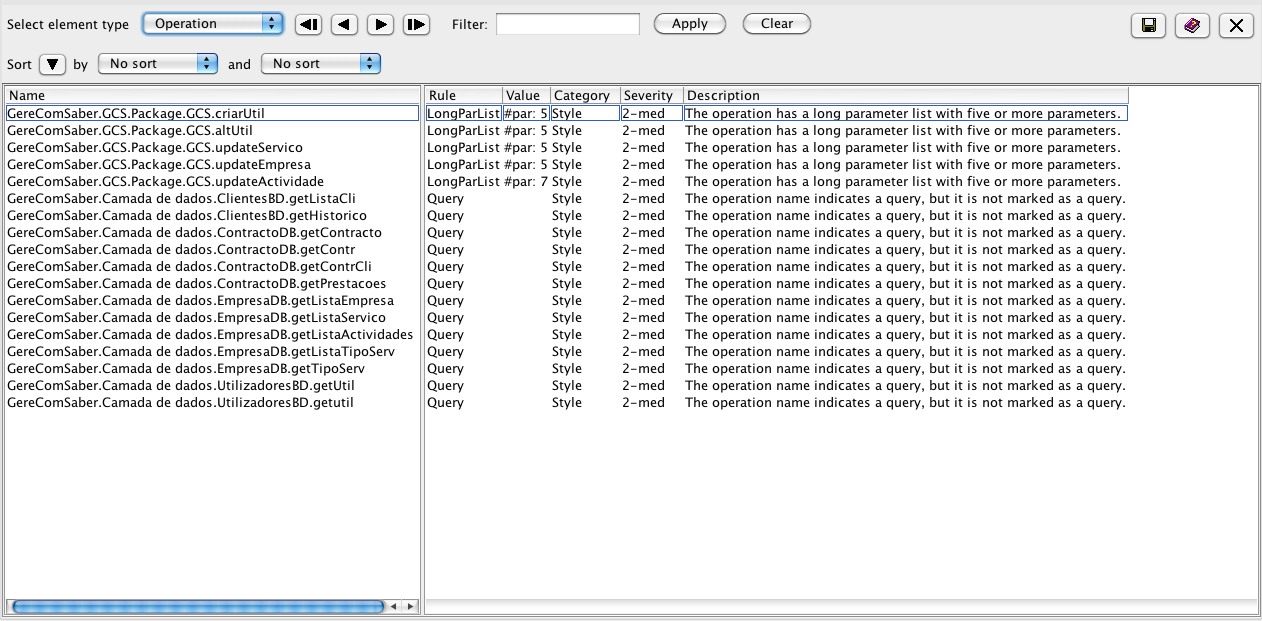
\includegraphics[width=1\textwidth]{images/rule.png}
\caption{Rule checking for Operations}\label{img:rule}
\end{center}
\end{figure} 

Based on the \textit{SDMetrics} manual, we will explain how to interpret each kind of metric, analysed by this software. \\
Size metrics, which usually count elements inside design elements (class, package, etc). The size metrics are good to estimate developing costs and effort. A large design element may indicate that it suffer's from poor design, resulting in low functional cohesion. This 	has a negative impact on the understandability, reusability, and maintainability of the design element. This size metrics can be directly found on the Metrics Table.\\
The coupling between design elements is also measured by \textit{SDMetrics}. Coupling is the degree to which the elements in a design are connected. The more the design elements are connected, the more they depend on each others. This high degree of dependency may affect the system maintainability, because when you change a design element, you may need to adapt the connected elements; and the system testability, because a problem in a design element may cause failure in a completly diferent conected element. Taking this in consideration, it is important to minimize coupling.\\
Inheritance-related metrics usually calculate features such as depth/width of the inheritance and number of ancestors/descendents of a design element. Such as high coupled elements, deep inheritance structures are believed to be more fault-prone. It is harder to fully understand a class that is situated deep in the inheritance tree, because you have to understand it's ancestor's. Also, modifying a design element with many descendants, may have a large impact on the system.\\
Complexity metrics measure the degree of connectivity between elements of a design element. They are concerned with relationships/dependencies between the elements in the design unit, such as the number of method invocations inside a class. The high complexity between the elements of a design element can make the design harder to understand, therefore more propitious to faults. Complexity metrics are usually strongly correlated with size measures. So even though they are good indicatures of quality, such as fault-proneness, they provide no new knowledge comparing to size metrics.\\
FALTA-ME FALAR DAS COHESION METRICS


 

%Sparkx Systems
\subsection{Sparx Systems Enterprise Architect}
\def \entArch {\textsf{Enterprise Architect}}
Sparx Systems \entArch\ is another tool that provides modeling of UML diagrams.
It supports mind map diagrams and project management, to provide full traceability from requirements specification to deployment end implementation.
This tool also provides some metrics evaluation to compute the complexity of a project based on Use Case diagrams. 

To perform this evaluation, the user needs to provide a level of implementation complexity for each interaction with authors. 
This task can be done when defining the Use Case descriptions or when performing the metrics evaluation.

To evaluate the metrics, \entArch\ has a wizard which enables other options for the complexity analysis.
These options manipulate the \emph{Technical} and the \emph{Environment} complexities and are used to adapt the evaluation and perform a better result on estimation.

Also can be filtered the Use Cases used in evaluation. 
To filter can be used manual selection or regular expressions over use case name.
This kind of filtering enables the project to be distributed and evaluated individually.
\subsubsection{Results}

To use this tool in metrics calculation, have the possibility do some tweaking over use case complexity, on their description, to get more precise results. This complexity admits simple values like low, medium or high.

Could also be edited some factors related to environment and technics complexity or hour rates in the wizard shown on the left side of Figure \ref{img:sparxRes}. Here we can use multiple factors to evaluate this factors, like usability or portability on technical complexity.

In the end we can access the Use Case metrics wizard and it is presented to us, as in the right side in Figure \ref{img:sparxRes}, the set of default values used to evaluate the effort of task.

\begin{figure}[H]
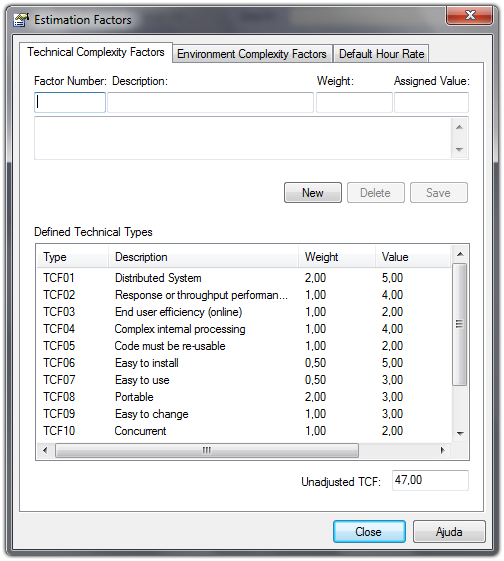
\includegraphics[scale=0.257]{images/sparxestim.png}
\hspace{0.1cm}
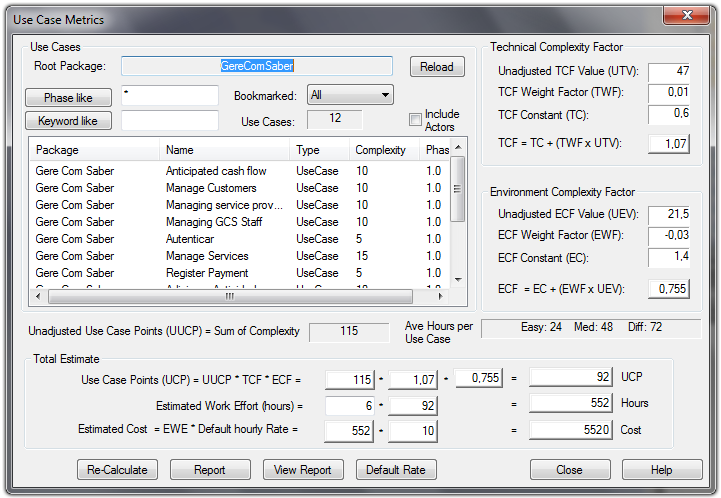
\includegraphics[scale=0.29]{images/sparx.png}
\caption{Estimation Factors and Use Case Metrics \entArch\ wizards}\label{img:sparxRes}
\end{figure}

The final result of metrics evaluation, is an estimation of Working Hours, Use Case Points\cite{Ribu01estimatingobject-oriented} and Total Cost needed to perform the development of system.

In Our case, because we have twelve Use Cases and had many of them with medium complexity. The effort to complete the task is 552 working hours, that would give a final result of \EUR{5.520}. 
To get this value only was changed the use cases complexity and everything else was left with default values.

%%Metrics Assessment
\section{Metrics Assessment}

\begin{quotation}
Effective management of any process requires quantification, measurement, and modeling. Software metrics provide a quantitative basis for the development and validation of models of the software development process. Metrics can be used to improve software productivity and quality.\cite{g1:Millis:1998}
\end{quotation}


--Entra o assunto da Secção 2 do artigo do Azevedo, JJ e Tiago.

    * Explicar aqui que as métricas não podem ser observadas, por si só, fora do contexto. Este problema prende-se essencialmente com o facto deste tipo de medições ser empírica, ou baseada em métodos empíricos.

    * Explicar em maior detalhe o que se entendo como validação de métricas (Kaner e Walter Bond).
%%Conclusão
\section{Conclusion} \label{conc}

In general, the software development process follows a systematic approach aiming the achievement of a quality system.
This software quality is not limited to the development of systems which respect several quality standards; it also ensures that the software fulfills all the specified requirements.
Thus, it became essential to include metrics on the software development lifecycle for monitoring its quality.
Most of the existing approaches involve a source code analysis and cannot be applied in earlier stages of the development process.
Applying metrics to \uml\ models enable an early estimate of development efforts, implementation time, complexity and cost of the system under development.
For this paper we focus our research on the most relevant metrics for this models and into testing two tools capable to measure them: \sdmetrics\ and  \entArch\ systems.

%A qualidade na ̃o passa apenas pela obtenc ̧a ̃o de software que respeita as diversas normas e padro ̃es de qualidade, mas tambe ́m pela garantia de que este cumpre todos os requisitos especificados. As medic ̧o ̃es quantitativas associadas a esta problema ́tica revelam-se essenciais em qualquer cieˆncia, o que na ̃o e ́ excepc ̧a ̃o na Engenharia de Software: existe um esforc ̧o cont ́ınuo para encontrar novas propostas, adequadas ao desenvolvimento de software. Com este artigo pretendemos assim mostrar como tirar partido das Linguagens de Modelac ̧a ̃o existentes, e aplicar estas medic ̧o ̃es qualitativas numa fase mais inicial do projecto (aquando a sua modelac ̧a ̃o), de forma a na ̃o centrar a ana ́lise apenas no co ́digo fonte. Apresentamos assim as principais me ́tricas existentes dentro da a ́rea da medic ̧a ̃o de modelos de UML e algumas das principais ferramentas para especificac ̧a ̃o de me ́tricas sobre UML, que combinado com a aplicac ̧a ̃o de me ́tricas tambe ́m ao co ́digo fonte se revela um aliado fundamental para uma melhor gesta ̃o do software produzido.

%SDMetrics
We can conclude that \sdmetrics\ is a versatile tool for calculate a large set of metrics over a wide range of \uml\ diagrams. Based on this metrics we can try to measure the quality and complexity of a software model.
It has an interesting GUI which provides several output views, from simple \emph{tables} to \emph{Histograms}. It finds potential problems with the model and also enables new metrics definition.

The major disadvantage of this tool is the inability of giving the user a plain and simple notion of the model quality, although \sdmetrics\ Manual provides simple tips of how to interpret each kind of metric -- crucial for a correct results reading.
At a glance, \sdmetrics\ results are guidelines for finding the good and the bad points of  \uml\ models, not a full specification of the models quality. 
%Although good documentation is provided,  which provide guidelines to the result interpretation.

On the other hand, \entArch\ is a full formal \uml\ specification environment that also supports metrics calculation oriented to Use Case diagrams. 
It is driven to enterprise market and oriented to minimize the cost and time spent with the production process.

This tool provides simple results and represents a good choice for have an estimation of the implementation cost on a formally specified system. 
With its system wizard, the user can adapt the value of the factors related to the environment and technics complexity for obtain an accurate estimation of the system final cost.
This requires some extra user interaction in the specification of a task complexity and a large knowledge of the system under development.
This complexity could be archived by other means if other types of diagrams were also analyzed.
Summing up, \entArch\  does not provide any kind of analysis about the quality of the model or do any automatic analysis about the system complexity: it estimates the final cost and effort of the project.

\begin{comment}
%bad
We consider this a valid approach, but it requires some extra user interaction in the specification of the complexity of a task.
This complexity could be archived by other means if other types of diagrams were also analyzed.
%good
The final results presented are simple and also oriented to the final cost, but if the complexity has been specified with knowledge of the environment, they could estimate very well the final cost of the implemented system.

Summing up, in metrics evaluation, this tool is a good choice to have an estimation of the implementation cost on a formally specified system, but this is its only goal, it cannot provide any kind of analysis about the quality of specification or do any automatic analysis about the system complexity.
\end{comment}


\section*{Acknowledgments}
The authors would like to thank to the SDMetrics staff for provide us an Academic License to explore the full system features presented in this document.
%%Biblio
\bibliographystyle{alpha}
\bibliography{modLangCorta11}


\end{document} 
